\documentclass[floatsintext,man]{apa6}

\usepackage{amssymb,amsmath}
\usepackage{ifxetex,ifluatex}
\usepackage{fixltx2e} % provides \textsubscript
\ifnum 0\ifxetex 1\fi\ifluatex 1\fi=0 % if pdftex
  \usepackage[T1]{fontenc}
  \usepackage[utf8]{inputenc}
\else % if luatex or xelatex
  \ifxetex
    \usepackage{mathspec}
    \usepackage{xltxtra,xunicode}
  \else
    \usepackage{fontspec}
  \fi
  \defaultfontfeatures{Mapping=tex-text,Scale=MatchLowercase}
  \newcommand{\euro}{€}
\fi
% use upquote if available, for straight quotes in verbatim environments
\IfFileExists{upquote.sty}{\usepackage{upquote}}{}
% use microtype if available
\IfFileExists{microtype.sty}{\usepackage{microtype}}{}

% Table formatting
\usepackage{longtable, booktabs}
\usepackage{lscape}
% \usepackage[counterclockwise]{rotating}   % Landscape page setup for large tables
\usepackage{multirow}		% Table styling
\usepackage{tabularx}		% Control Column width
\usepackage[flushleft]{threeparttable}	% Allows for three part tables with a specified notes section
\usepackage{threeparttablex}            % Lets threeparttable work with longtable

% Create new environments so endfloat can handle them
% \newenvironment{ltable}
%   {\begin{landscape}\begin{center}\begin{threeparttable}}
%   {\end{threeparttable}\end{center}\end{landscape}}

\newenvironment{lltable}
  {\begin{landscape}\begin{center}\begin{ThreePartTable}}
  {\end{ThreePartTable}\end{center}\end{landscape}}




% The following enables adjusting longtable caption width to table width
% Solution found at http://golatex.de/longtable-mit-caption-so-breit-wie-die-tabelle-t15767.html
\makeatletter
\newcommand\LastLTentrywidth{1em}
\newlength\longtablewidth
\setlength{\longtablewidth}{1in}
\newcommand\getlongtablewidth{%
 \begingroup
  \ifcsname LT@\roman{LT@tables}\endcsname
  \global\longtablewidth=0pt
  \renewcommand\LT@entry[2]{\global\advance\longtablewidth by ##2\relax\gdef\LastLTentrywidth{##2}}%
  \@nameuse{LT@\roman{LT@tables}}%
  \fi
\endgroup}


  \usepackage{graphicx}
  \makeatletter
  \def\maxwidth{\ifdim\Gin@nat@width>\linewidth\linewidth\else\Gin@nat@width\fi}
  \def\maxheight{\ifdim\Gin@nat@height>\textheight\textheight\else\Gin@nat@height\fi}
  \makeatother
  % Scale images if necessary, so that they will not overflow the page
  % margins by default, and it is still possible to overwrite the defaults
  % using explicit options in \includegraphics[width, height, ...]{}
  \setkeys{Gin}{width=\maxwidth,height=\maxheight,keepaspectratio}
\ifxetex
  \usepackage[setpagesize=false, % page size defined by xetex
              unicode=false, % unicode breaks when used with xetex
              xetex]{hyperref}
\else
  \usepackage[unicode=true]{hyperref}
\fi
\hypersetup{breaklinks=true,
            pdfauthor={},
            pdftitle={Linking hypothesis and number of response options modulate inferred scalar implicature rate},
            colorlinks=true,
            citecolor=blue,
            urlcolor=blue,
            linkcolor=black,
            pdfborder={0 0 0}}
\urlstyle{same}  % don't use monospace font for urls

\setlength{\parindent}{0pt}
%\setlength{\parskip}{0pt plus 0pt minus 0pt}

\setlength{\emergencystretch}{3em}  % prevent overfull lines


% Manuscript styling
\captionsetup{font=singlespacing,justification=justified}
\usepackage{csquotes}
\usepackage{upgreek}

 % Line numbering
  \usepackage{lineno}
  \linenumbers


\usepackage{tikz} % Variable definition to generate author note

% fix for \tightlist problem in pandoc 1.14
\providecommand{\tightlist}{%
  \setlength{\itemsep}{0pt}\setlength{\parskip}{0pt}}

% Essential manuscript parts
  \title{Linking hypothesis and number of response options modulate inferred
scalar implicature rate}

  \shorttitle{Linking hypotheses and implicature rate}


  \author{Masoud Jasbi\textsuperscript{1}, Brandon Waldon\textsuperscript{1}, \& Judith Degen\textsuperscript{1}}

  % \def\affdep{{"", "", ""}}%
  % \def\affcity{{"", "", ""}}%

  \affiliation{
    \vspace{0.5cm}
          \textsuperscript{1} Stanford University  }

  \authornote{
    XXX Add complete departmental affiliations for each author here. Each
    new line herein must be indented, like this line. Enter author note
    here.
    
    Correspondence concerning this article should be addressed to Masoud
    Jasbi, XXX Postal address. E-mail: XXX
    \href{mailto:my@email.com}{\nolinkurl{my@email.com}}
  }


  \abstract{The past 15 years have seen increasing experimental investigations of
core pragmatic questions in the ever more active and lively field of
experimental pragmatics. Within experimental pragmatics, many of the
core questions have relied on the operationalization of the theoretical
notion of `implicature rate'. Implicature rate based results have
informed the work on acquisition, online processing, and scalar
diversity, inter alia. Despite its theoretical importance. Implicature
rate has typically been quantified as the proportion of `pragmatic'
judgments in two-alternative forced choice truth value judgment tasks.
Despite its theoretical importance, this linking hypothesis from
implicature rate to behavioral responses has never been extensively
tested. Here we show that two factors dramatically affect the
`implicature rate' inferred from truth value judgment tasks: a) the
number of responses provided to participants; and b) the linking
hypothesis about what constitutes a `pragmatic' judgment. We argue that
it is time for the field of experimental pragmatics to engage more
seriously with its foundational assumptions about how theoretical
notions map onto behaviorally measurable quantities, and present a
sketch of an alternative linking hypothesis that derives behavior in
truth value judgment tasks from probabilistic utterance expectations.}
  \keywords{scalar implicature; methodology; linking hypothesis; experimental
pragmatics; truth value judgment task \\

    \indent Word count: X
  }





\usepackage{amsthm}
\newtheorem{theorem}{Theorem}[section]
\newtheorem{lemma}{Lemma}[section]
\theoremstyle{definition}
\newtheorem{definition}{Definition}[section]
\newtheorem{corollary}{Corollary}[section]
\newtheorem{proposition}{Proposition}[section]
\theoremstyle{definition}
\newtheorem{example}{Example}[section]
\theoremstyle{definition}
\newtheorem{exercise}{Exercise}[section]
\theoremstyle{remark}
\newtheorem*{remark}{Remark}
\newtheorem*{solution}{Solution}
\begin{document}

\maketitle

\setcounter{secnumdepth}{0}



\section{Introduction}\label{introduction}

The past 15 years have seen the rise and development of a bustling and
exciting new field at the intersection of linguistics, psychology, and
philosophy: \emph{experimental pragmatics} (Barner, Brooks, \& Bale,
2011; Bonnefon, Feeney, \& Villejoubert, 2009; Bott \& Chemla, 2016;
Bott \& Noveck, 2004; Breheny, Ferguson, \& Katsos, 2013; Breheny,
Katsos, \& Williams, 2006; Chierchia et al., 2001; De Neys \& Schaeken,
2007; Degen \& Tanenhaus, 2015, 2016; Geurts \& Pouscoulous, 2009;
Grodner, Klein, Carbary, \& Tanenhaus, 2010; Huang \& Snedeker, 2009;
Katsos \& Bishop, 2011; I. A. Noveck \& Reboul, 2008; Noveck \& Posada,
2003; Papafragou \& Tantalou, 2004; Tiel, Miltenburg, Zevakhina, \&
Geurts, 2014; Tomlinson, Bailey, \& Bott, 2013). Experimental pragmatics
is devoted to experimentally testing theories of how language is used in
context. How do listeners draw inferences about the -- often
underspecified -- linguistic signal they receive from speakers? How do
speakers choose between the many utterance alternatives they have at
their disposal?

The most prominently studied phenomenon in experimental pragmatics is
undoubtedly \emph{scalar implicature}. Scalar implicatures arise as a
result of a speaker producing the weaker of two ordered scalemates
(Geurts, 2010; Grice, 1975; Hirschberg, 1985; Horn, 1972). Examples are
provided in (1-2).

\begin{enumerate}
\def\labelenumi{\arabic{enumi}.}
\item
\end{enumerate}

\begin{itemize}
\tightlist
\item
  \emph{Utterance:} Some of her pets are cats.
\item
  \emph{Implicature:} Some, but not all, of her pets are cats.
\item
  \emph{Scale:} 
\end{itemize}

\begin{enumerate}
\def\labelenumi{\arabic{enumi}.}
\setcounter{enumi}{1}
\item
\end{enumerate}

\begin{itemize}
\tightlist
\item
  \emph{Utterance:} She owns a cat or a dog.
\item
  \emph{Implicature:} She owns a cat or a dog, but not both.
\item
  \emph{Scale:} 
\end{itemize}

A listener, upon observing the utterances in (1-2a) typically infers
that the speaker intended to convey the meanings in (1-2b),
respectively. Since Grice (1975), the agreed-upon abstract
rationalization the listener could give for their inference goes
something like this: the speaker could have made a more informative
statement by producing the stronger alternative (e.g., \emph{All of her
pets are cats.} in (1)). If the stronger alternative is true, they
should have produced it to comply with the Cooperative Principle. They
chose not to. I believe the speaker knows whether the stronger
alternative is true. Hence, it must not be true. The derivation
procedure for ad hoc exhaustive inferences such as in (3) is assumed to
be calculable in the same way as for scalar implicatures, though the
scale is assumed to be contextually driven.

Because the basic reconstruction of the inference is much more easily
characterized for scalar implicatures than for other implicatures,
scalar implicatures have served as a test bed for many questions in
experimental pragmatics, including, but not limited to:

\begin{enumerate}
\def\labelenumi{\arabic{enumi}.}
\item
  Are scalar inferences default inferences, in the sense that they arise
  unless blocked by (marked) contexts (Degen, 2015; Horn, 1984;
  Levinson, 2000)?
\item
  Are scalar inferences default inferences, in the sense that they are
  computed automatically in online processing and only cancelled by
  context in a second effortful step if required by context) (Bott \&
  Noveck, 2004; Breheny et al., 2006; Degen \& Tanenhaus, 2016; Grodner
  et al., 2010; Huang \& Snedeker, 2009; Politzer-Ahles \& Fiorentino,
  2013; Tomlinson et al., 2013)?
\item
  What are the (linguistic and extra-linguistic) factors that affect
  whether a scalar implicature is derived (Bergen \& Grodner, 2012;
  Bonnefon et al., 2009; Breheny et al., 2013, 2006; Chemla \& Spector,
  2011; De Neys \& Schaeken, 2007; Degen, 2015; Degen \& Goodman, 2014;
  Degen \& Tanenhaus, 2015, 2016; Marneffe \& Tonhauser, 2016; Potts,
  Lassiter, Levy, \& Frank, 2015; Zondervan, 2010)?
\item
  How much diversity is there across implicature types, and within
  scalar implicatures across scale types, in whether or not an
  implicature is computed (Doran, Ward, Larson, McNabb, \& Baker, 2012;
  Tiel et al., 2014)?
\item
  At what age do children acquire the ability to compute implicatures
  (Barner et al., 2011; Horowitz, Schneider, \& Frank, 2017; Katsos \&
  Bishop, 2011; Musolino, 2004; Noveck, 2001; Papafragou \& Tantalou,
  2004; Stiller, Goodman, \& Frank, 2015)?
\end{enumerate}

In addressing all of these questions, it has been crucial to obtain
estimates of \emph{implicature rates}. For 1., implicature rates from
experimental tasks can be taken to inform whether scalar implicatures
should be considered default inferences. For 2., processing measures on
responses that indicate implicatures can be compared to processing
measures on responses that indicate literal interpretations. For 3.,
contextual effects can be examined by comparing implicature rates across
contexts. For 4., implicature rates can be compared across scales (or
across implicature types). For 5., implicature rates can be compared
across age groups.

A standard measure that has stood as a proxy for implicature rate across
many studies is the proportion of \enquote{pragmatic} judgments in truth
value judgment paradigms (Bott \& Noveck, 2004; Chemla \& Spector, 2011;
De Neys \& Schaeken, 2007; Degen \& Goodman, 2014; Degen \& Tanenhaus,
2015; Geurts \& Pouscoulous, 2009; Noveck, 2001; Noveck \& Posada,
2003). In these kinds of tasks, participants are provided a set of
facts, either presented visually or via their own knowledge of the
world. They are then asked to judge whether a sentence intended to
describe those facts is true or false (or alternatively, whether it is
right or wrong, or they are asked whether they agree or disagree with
the sentence). The crucial condition for assessing implicature rates in
these kinds of studies typically consists of a case where the facts are
such that the stronger alternative is true and the target utterance is
thus also true but underinformative. For instance, Bott and Noveck
(2004) asked participants to judge sentences like \enquote{Some
elephants are mammals}, when world knowledge dictates that all elephants
are mammals. Similarly, Degen and Tanenhaus (2015) asked participants to
judge sentences like \enquote{You got some of the gumballs} in
situations where the visual evidence indicated that the participant
received all the gumballs from a gumball machine. In these kinds of
scenarios, the story goes, if a participant responds \enquote{FALSE},
that indicates that they computed a scalar implicature, eg to the effect
of \enquote{Not all elephants are mammals} or \enquote{You didn't get
all of the gumballs}, which is (globally or contextually) false. If
instead a participant responds \enquote{TRUE}, that is taken to indicate
that they interpreted the utterance literally as `Some, and possibly
all, elephants are mammals' or \enquote{You got some, and possibly all,
of the gumballs}.

Given the centrality of the theoretical notion of \enquote{implicature
rate} to much of experimental pragmatics, there is to date a surprising
lack of discussion of the basic assumption that it is adequately
captured by the proportion of FALSE responses in truth value judgment
tasks (but see Benz and Gotzner (2014); Geurts and Pouscoulous (2009);
Degen and Goodman (2014); Katsos and Bishop (2011)). Indeed, the scalar
implicature acquisition literature was shaken up when Katsos and Bishop
(2011) showed that simply by introducing an additional response option,
children started looking much more pragmatic than had been previously
observed in a binary judgment paradigm. Katsos and Bishop (2011) allowed
children to distribute 1, 2, or 3 strawberries to a puppet depending on
\enquote{how good the puppet said it}. The result was that children gave
on average fewer strawberries to the puppet when he produced
underinformative utterances compared to when he produced literally true
and pragmatically felicitous utterances, suggesting that children do, in
fact, display pragmatic ability even at ages when they had previously
appeared not to.

But this raises an important question: in truth value judgment tasks,
how does the researcher know whether an interpretation is literal or the
result of an implicature computation? The binary choice task typically
used is appealing in part because it allows for a direct mapping from
response options -- TRUE and FALSE -- to interpretations -- literal and
pragmatic. That the seeming simplicity of this mapping is illusory
becomes apparent once a third response option is introduced, as in the
Katsos and Bishop (2011) case. How is the researcher to interpret the
intermediate option? Katsos and Bishop (2011) grouped the intermediate
option with the negative endpoint of the scale for the purpose of
categorizing judgments as literal vs.~pragmatic, i.e., they interpreted
the intermediate option as pragmatic. But it seems just as plausible
that they could have grouped it with the positive endpoint of the scale
and taken the hard line that only truly FALSE responses constitute
evidence of a full-fledged implicature. The point here is that there has
been remarkably little consideration of \emph{linking hypothesiss}
between behavioral measures and theoretical constructs in experimental
pragmatics, a problem in many subfields of psycholinguistics (Tanenhaus,
2004). We argue that it is time to engage more seriously with these
issues.

We begin by reporting an experiment that addresses the following
question: do the number of response options provided in a truth value
judgment task and the way that responses are grouped into pragmatic
(\enquote{SI}) and literal (\enquote{no SI}) change inferences about
scalar implicature rates? Note that this way of asking the question
presupposes two things: first, that whatever participants are doing in a
truth value judgment task, the behavioral measure can be interpreted as
providing a measure of interpretation; and second, that listeners either
do or do not compute an implicature on any given occasion. In the
General Discussion we will discuss both of these issues. First,
following Degen and Goodman (2014), we will offer some remarks on why
truth value judgment tasks are better thought of as measuring
participants' estimates of speakers' \emph{production} probabilities.
This will suggest a completely different class of linking hypothesiss.
Next, we discuss an alternative conception of scalar implicature as a
probabilistic phenomeonen, a view that has recently rose to prominence
in the subfield of probabilistic pragmatics (Franke \& Jäger, 2016;
Goodman \& Frank, 2016). This alternative conception of scalar
implicature, we argue, affords developing and testing quantitative
linking hypothesiss in a rigorous and motivated way.

Consider a setup in which a listener is presented a card with a
depiction of either one or two animals (see Figure
\ref{fig:linkvisualization} for an example). As in a standard truth
value judgment task, the listener then observes an underinformative
utterance about this card (e.g., \enquote{There is a cat or a dog on the
card}) and is asked to provide a judgment on a scale with 2, 3, 4, or 5
response options, with endpoints \enquote{wrong} and
\enquote{right.}\footnote{An open question concerns the extent to which
  the labeling of points on the scale affects judgments (e.g.,
  \enquote{wrong}--\enquote{right} vs. \enquote{false}--\enquote{true}
  vs. \enquote{disagree}--\enquote{agree}). While some studies have used
  \enquote{false}--\enquote{true}, others have argued that judging truth
  may lead to meta-linguistic reasoning in participants that could
  distort judgments.} In the binary case, this reproduces the standard
truth value judgment task. Figure \ref{fig:linkvisualization}
exemplifies (some of) the researcher's options for grouping responses.
Under what we will call the \enquote{Strong link} assumption, only the
negative endpoint of the scale is interpreted as evidence for a scalar
implicature having been computed. Under the \enquote{Weak link}
assumption, in contrast, any response that does not correspond to the
positive endpoint of the scale is interpreted as evidence for a scalar
implicature having been computed. Intermediate grouping schemes are also
possible, but these are the ones we will consider here. Note that for
the binary case, the Weak and Strong link return the same categorization
scheme, but for any number of response options greater than 2, the Weak
and Strong link can in principle lead to differences in inferences about
implicature rate.

\begin{figure}
\centering
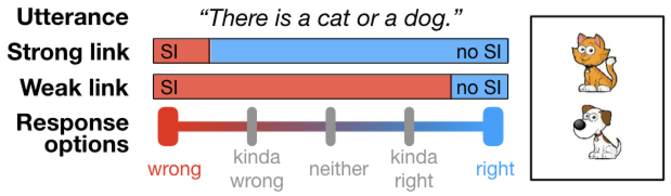
\includegraphics{writeup_files/figure-latex/linkvisualization-1.pdf}
\caption{\label{fig:linkvisualization}Strong and Weak link from response
options to researcher inference about scalar implicature rate,
exemplified for the disjunctive utterance when the conjunction is true.}
\end{figure}

Let's examine an example. Assume three response options (wrong, neither,
right). Assume further that each of the three responses was selected by
a third of participants, i.e., the distributions of responses is 1/3,
1/3, and 1/3. Under the Strong link, we infer that this task yielded an
implicature rate of 2/3. Under the Weak link, we infer that this task
yielded an implicature rate of 1/3. This is quite a drastic difference
if we are, for instance, interested in whether scalar implicatures are
inference defaults and we would like to interpret an implicature rate of
above an arbitrary threshold (e.g., 50\%) as evidence for such a claim.
Under the Strong link, we would conclude that scalar implicatures are
not defaults. Under the Weak link, we would conclude that they are. In
the experiment reported in the following section, we presented
participants with exactly this setup. We manipulated the number of
response options between participants and analyzed the results under
different linking hypothesiss.

\section{Experiment}\label{experiment}

Participants played an online card game in which they were asked to
judge descriptions of the contents of cards. Different groups of
participants were presented with different numbers of response options.
On critical trials, participants were presented with descriptions for
the cards that typically result in exhaustivity implicatures
(\enquote{There is a cat on the card} when there was a cat and a dog) or
scalar implicatures (\enquote{There is a cat or a dog on the card} when
there was a cat and a dog). We categorized their responses on such
trials according to the weak and the Strong link introduced above, and
tested whether the number of response options and the linking
hypothesiss led to different conclusions about the rate of computed
implicatures in the experimental task.

\subsection{Methods}\label{methods}

\subsubsection{Participants}\label{participants}

200 participants were recruited via Amazon Mechanical Turk. They
optionally provided demographic information at the end of the study.
Participants' mean age was 35. We also asked participants if they had
any prior training in logic. 40 participants reported that they did,
while 160 had no prior training in logic. All participants' data was
included in the final analysis.

\subsubsection{Materials and procedure}\label{materials-and-procedure}

The study was administered online through Amazon Mechanical
Turk.\footnote{The experiment can be viewed
  \href{https://cdn.rawgit.com/thegricean/si-paradigms/94a590f0/experiments/main/1_methods/online_experiment/connective_game.html}{here}.}
Participants were first introduced to the set of cards we used in the
study (Figure \ref{fig:stimuli}). Each card depicted one or two animals,
where an animal could be either a cat, a dog, or an elephant. Then
participants were introduced to a blindfolded fictional character called
Bob. Bob was blindfolded to avoid violations of ignorance expectations
associated with the use of disjunction ({\textbf{???}}; Chierchia et
al., 2001) Participants were told that Bob would guess the contents of
the cards and their task was to indicate whether Bob's guess was wrong
or right. On each trial, participants saw a card and a sentence
representing Bob's guess. For example, they saw a card with a cat and
read the sentence \enquote{There is a cat on the card.} They then
provided an assessment of Bob's guess. The study ended after 24 trials.

\begin{figure}
\centering
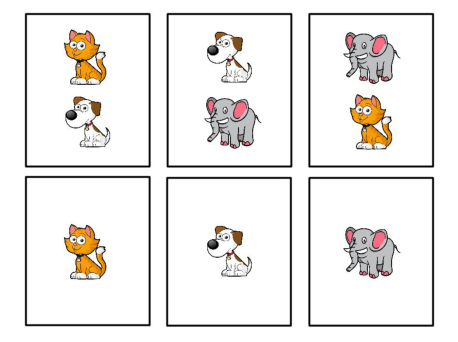
\includegraphics{writeup_files/figure-latex/stimuli-1.pdf}
\caption{\label{fig:stimuli}Cards used in the connective guessing game.}
\end{figure}

Two factors were manipulated within participants: card type and guess
type. There were two types of cards, cards with only one animal on them
and cards with two animals. There were three types of guesses: simple
(e.g. \emph{There is a cat}), conjunctive (e.g. \emph{There is a cat and
a dog}), and disjunctive (e.g. \emph{There is a cat or a dog}). Crossing
card type and guess type yielded trials of varying theoretical interest
(see Figure \ref{fig:trials}): critical underinformative trials that
were likely to elicit pragmatic inferences (either scalar or exhaustive)
and control trials that were either unambiguously true or false. Each
trial type occurred three times with randomly sampled animals and
utterances that satisfied the constraint of the trial type. Trial order
was randomized.

\begin{figure}
\centering
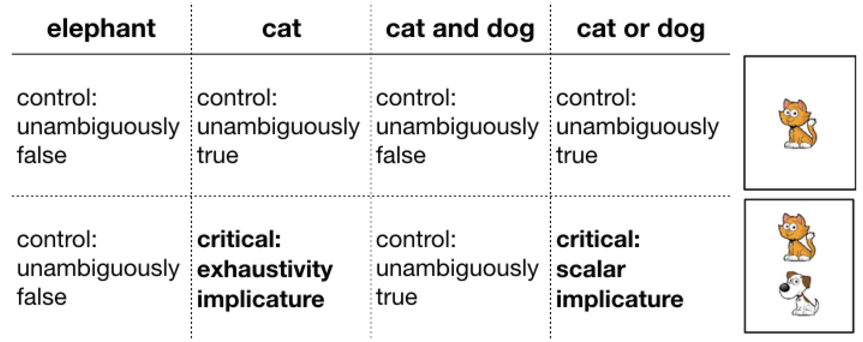
\includegraphics{writeup_files/figure-latex/trials-1.pdf}
\caption{\label{fig:trials}Trial types (critical and control). Headers
indicate utterance types. Rows indicate card types. Critical trials are
marked in bold.}
\end{figure}

On critical trials, participants could derive implicatures in two ways.
First, on trials on which two animals were present on the card (e.g.,
cat and dog) but Bob guessed only one of them (e.g. \enquote{There is a
cat on the card}), the utterance could have a literal interpretation
(\enquote{There is a cat and possibly another animal on the card}) or an
exhaustive interpretation (\enquote{There is only a cat on the card}).
We refer to these trials as \enquote{exhaustive}. Second, on trials on
which two animals were on the card (e.g., a cat and a dog) and Bob used
a disjunciton (e.g., \enquote{There is a cat or a dog on the card}), the
utterance could have the literal, inclusive, interpretation, or a
pragmatic, exclusive interpretation. We refer to these trials as
\enquote{scalar}.

In order to assess the effect of the number of response options on
implicature rate, we manipulated number of response options in the
forced choice task between participants. We refer to the choice
conditions as \enquote{binary} (options: \emph{wrong}, \emph{right}),
\enquote{ternary} (options: \emph{wrong}, \emph{neither}, \emph{right}),
\enquote{quaternary} (options: \emph{wrong}, \emph{kinda wrong},
\emph{kinda right}, \emph{right}), and \enquote{quinary} (\emph{wrong},
\emph{kinda wrong}, \emph{neither}, \emph{kinda right}, \emph{right}).
Thus, the endpoint labels always remained the same. If there was an
uneven number of response options, the central option was
\emph{neither}. Participants were randomly assigned to one of the four
task conditions.

\subsection{Results and discussion}\label{results-and-discussion}

The collected dataset contains 50 participants in the binary task, 53 in
the ternary task, 43 in the quaternary task, and 54 in the quinary task.
Figures \ref{fig:binaryPlot} to \ref{fig:quinaryPlot} show the
proportions of response choices in each of the 8 trial types on each of
the four response tasks, respectively. We report the relevant patterns
of results qualitatively before turning to the quantitative analysis of
interest.

\subsubsection{Qualitative analysis}\label{qualitative-analysis}

\begin{figure}
\centering
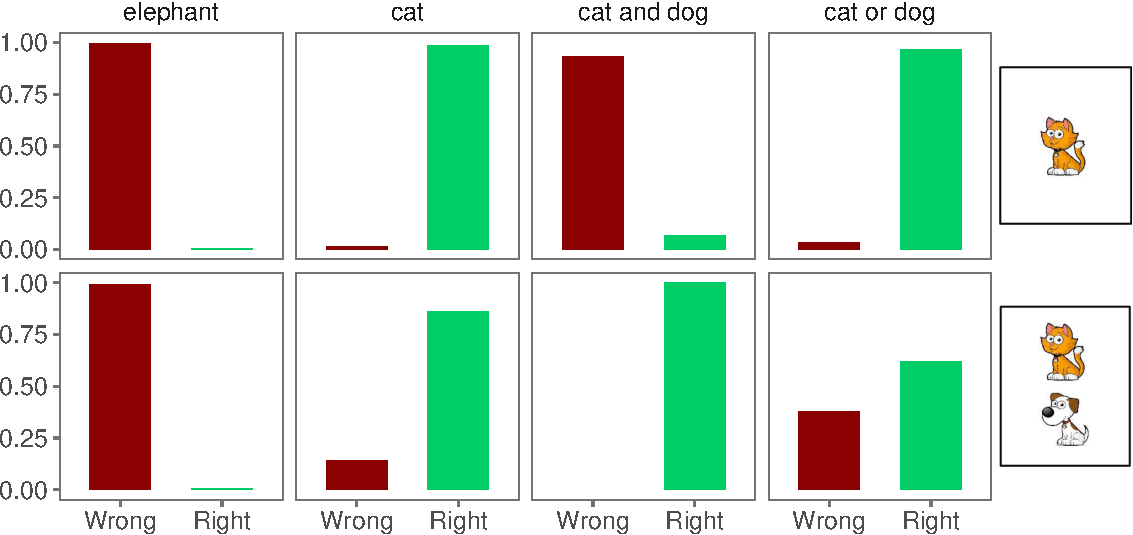
\includegraphics{writeup_files/figure-latex/binaryPlot-1.pdf}
\caption{\label{fig:binaryPlot}Proportion of responses for the binary forced
choice judgments. Error bars indicate 95\% bootstrapped confidence
intervals.}
\end{figure}

In the binary task, participants were at or close to ceiling in
responding \enquote{right} and \enquote{wrong} on unambiguously true and
false trials, respectively (see Figure \ref{fig:binaryPlot}). However,
on underinformative trials (i.e.~a \enquote{cat} or \enquote{cat or dog}
description for a card with both a cat and a dog), we observe pragmatic
behavior: on exhaustive trials, participants judged the utterance
\enquote{wrong} 14\% of the time; on scalar trials, participants judged
the utterance \enquote{wrong} 38\% of the time. That is, both under the
Weak and Strong link assumptions introduced in the Introduction,
inferred implicature rate on exhaustive trials is 14\% and on scalar
trials 38\%.

\begin{figure}
\centering
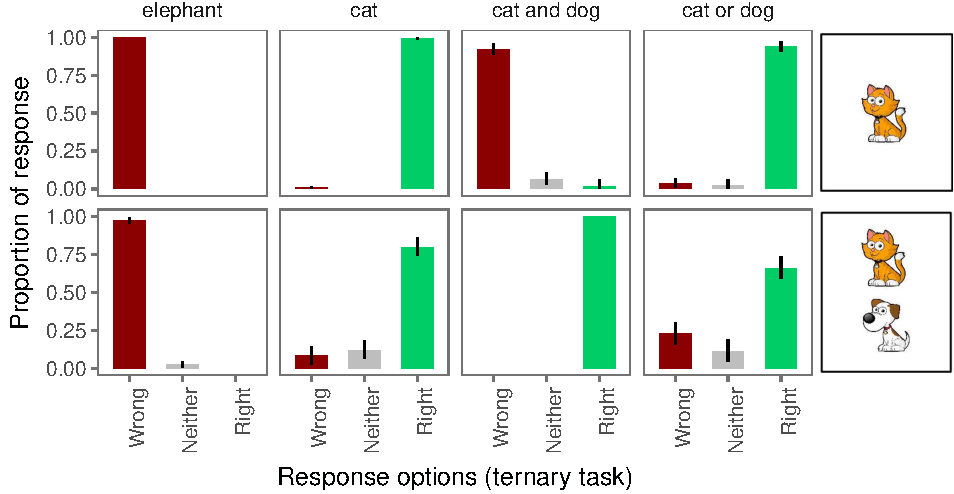
\includegraphics{writeup_files/figure-latex/ternaryPlot-1.pdf}
\caption{\label{fig:ternaryPlot}Proportion of responses for the ternary
forced choice judgments. Error bars indicate 95\% bootstrapped
confidence intervals.}
\end{figure}

In the ternary task, participants were also at or close to ceiling in
responding \enquote{right} and \enquote{wrong} on unambiguously true and
false trials, respectively (see Figure \ref{fig:ternaryPlot}). And
again, on underinformative trials (a \enquote{cat} and \enquote{cat or
dog} description for a card with both a cat and a dog), we observed
pragmatic behavior: on exhaustive trials, participants considered the
guess \enquote{wrong} 8\% of the time and neither wrong nor right 12\%
of the time. On scalar trials, participants judged the guess
\enquote{wrong} 23\% of the time and \enquote{neither} 11\% of the time.
This means that the Weak and Strong link lead to different conclusions
about implicature rates on the ternary task. Under the Weak link,
inferred implicature rate on exhaustive trials is 20\%; under the Strong
link it is only 8\%. Similarly, under the Weak link, inferred
implicature rate on scalar trials is 34\%; under the Strong link it is
only 23\%.

\begin{figure}
\centering
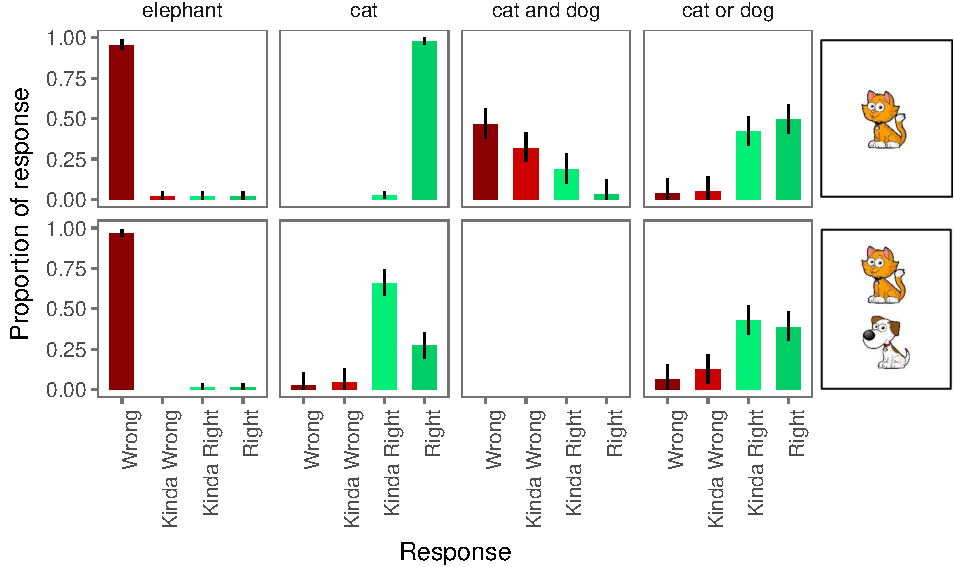
\includegraphics{writeup_files/figure-latex/quaternaryPlot-1.pdf}
\caption{\label{fig:quaternaryPlot}Proportion of responses for the
quaternary forced choice judgments. Error bars indicate 95\%
bootstrapped confidence intervals.}
\end{figure}

In the quaternary task (Figure \ref{fig:quaternaryPlot}), participants
were again at or close to ceiling in responding \enquote{right} and
\enquote{wrong} on 4 of the 6 unambiguously true and false trials.
However, with four response options, two of the control conditions
appear to be showing signs of pragmatic infelicity: when a conjunction
was used and only one of the animals was on the card, participants
considered the guess \enquote{wrong} most of the time, but they often
considered it \enquote{kinda wrong} or even \enquote{kinda right}. This
suggests that perhaps participants considered the notion of a partially
true or correct statement in our experimental setting. Disjunctive
descriptions of cards with only one animal, while previously at ceiling
for \enquote{right} responses, were downgraded to only \enquote{kinda
right} 26\% of the time, presumably because these utterances are also
underinformative, though the degree of underinformativeness may be less
egregious than on scalar trials.

On underinformative exhaustive trials, we observed pragmatic behavior as
before: participants judged the guess \enquote{wrong} 2\% of the time,
\enquote{kinda wrong} 5\% of the time, and \enquote{kinda right} 66\% of
the time. On scalar trials, participants judged the guess
\enquote{wrong} 6\% of the time, \enquote{kinda wrong} 12\% of the time,
and \enquote{kinda right} 43\% of the times.

Thus, we are again forced to draw different conclusions about
implicature rates depending on whether we assume the Weak link or the
Strong link. Under the Weak link, inferred implicature rate on
exhaustive trials is 73\%; under the Strong link it is only 2\%.
Similarly, under the Weak link, inferred implicature rate on scalar
trials is 61\%; under the Strong link it is only 6\%.

\begin{figure}
\centering
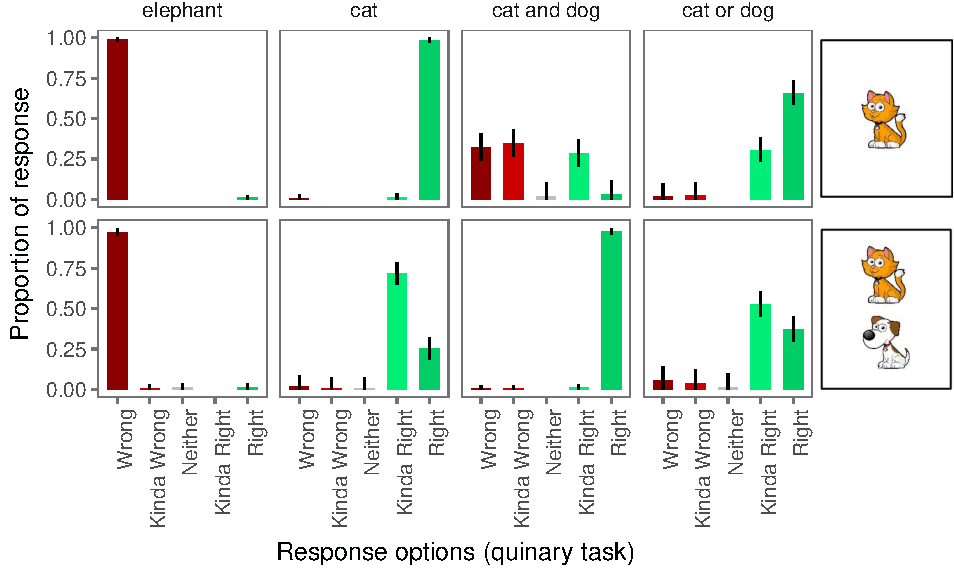
\includegraphics{writeup_files/figure-latex/quinaryPlot-1.pdf}
\caption{\label{fig:quinaryPlot}Proportion of responses for the quinary
forced choice judgments. Error bars indicate 95\% bootstrapped
confidence intervals.}
\end{figure}

Finally, Figure \ref{fig:quinaryPlot} shows the proportion of responses
in the quinary task. Performance on the 4 pragmatically felicitous
control trials was again at floor and ceiling, respectively. The 2
control conditions in which the quaternary task had revealed pragmatic
infelicity again displayed that pragmatic infelicity in the quinary
task, suggesting that this is a robust type of pragmatic infelicity
that, nonetheless, requires fine-grained enough response options to be
detected experimentally.

On underinformative exhaustive trials, we observed pragmatic behavior as
before: participants judged the guess \enquote{wrong} 2\% of the time,
\enquote{kinda wrong} 1 and 1\% of the time, \enquote{neither} 1 and 1\%
of the time, and \enquote{kinda right} 72\% of the time. On scalar
trials, participants judged the guess \enquote{wrong} 6\% of the time,
\enquote{kinda wrong} 4\% of the time, \enquote{neither} 1\% of the
time, and \enquote{kinda right} 52\% of the time.

Thus, we would again draw different conclusions about implicature rates
depending on whether we assume the Weak link or the Strong link. Under
the Weak link, inferred implicature rate on exhaustive trials is 76 and
76\%; under the Strong link it is only 2\%. Similarly, under the Weak
link, inferred implicature rate on scalar trials is 63\%; under the
Strong link it is only 6\%.

\subsubsection{Quantitative analysis}\label{quantitative-analysis}

Our primary goal in this study was to test whether the estimated
implicature rate in the experimental task is affected by the linking
hypothesis and the number of response options available to participants.
To this end, we only analyzed the critical trials (exhaustive and
scalar). In particular, we classified each data point from critical
trials as constituting an implicature (1) or not (0) under the Strong
and Weak link. Figure \ref{fig:implicatureRatePlot} shows the resulting
implicature rates by condition and link.

Visually, the Weak link tends to result in greater estimates of
implicature rates, especially in tasks with more response options. Under
the Strong link, this latter pattern is reversed: the binary and ternary
judgment tasks result in greater estimates of implicature rates than
with more response options.

\begin{figure}
\centering
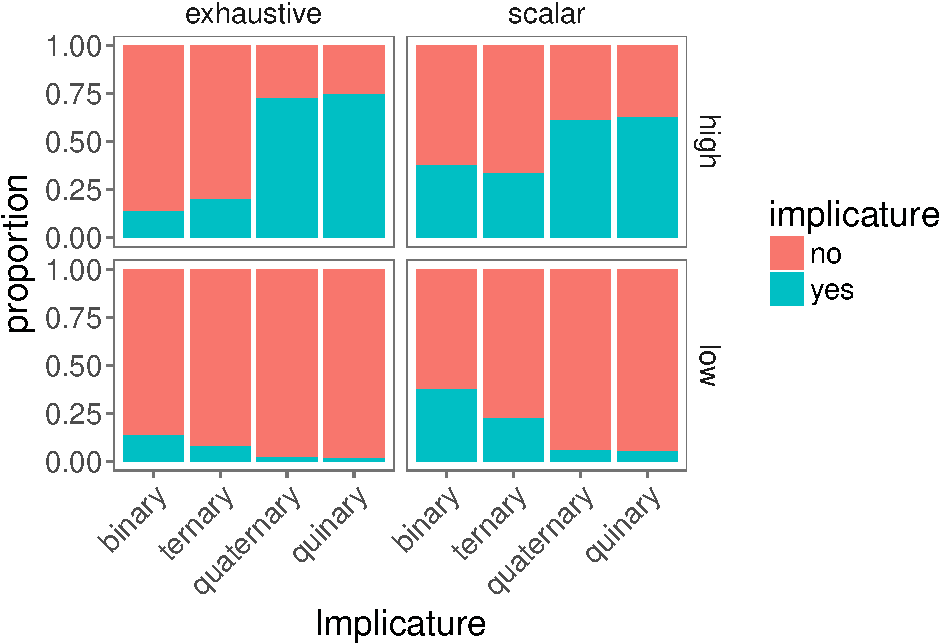
\includegraphics{writeup_files/figure-latex/implicatureRatePlot-1.pdf}
\caption{\label{fig:implicatureRatePlot}Inferred implicature rates on
exhaustive and scalar trials as obtained with the binary, ternary,
quaternary, and quinary response task. Columns indicate link from
response to implicature rate (strong: proportion of \enquote{wrong
judgments; weak: proportion of non-'right} judgments).}
\end{figure}

\begin{table}

\caption{\label{tab:implicatureRate}\label{tab:modeltable}Model parameter estimates and their credible intervals. Rows marked with an asterisk in the evidence column do not contain 0 in the credible interval, thereby providing evidence for an effect.}
\centering
\begin{tabular}[t]{lrrrl}
\toprule
Predictors & Estimate & 2.5\% & 97.5\% & Evidence\\
\midrule
Intercept & -8.60 & -13.98 & -4.53 & *\\
Link = Weak & -0.15 & -4.86 & 4.77 & \\
Task = Quaternary & -1.83 & -8.08 & 4.20 & \\
Task = Quinary & -4.05 & -10.90 & 2.38 & \\
Task = Ternary & -1.45 & -7.31 & 4.56 & \\
\addlinespace
Implicature = Scalar & 6.09 & 1.00 & 12.29 & *\\
Link = Weak : Task = Quaternary & 14.03 & 7.24 & 21.88 & *\\
Link = Weak : Task = Quinary & 17.28 & 10.64 & 25.80 & *\\
Link = Weak : Task = Ternary & 3.81 & -1.49 & 9.22 & \\
Link = Weak : Implicature = Scalar & 0.90 & -4.01 & 6.43 & \\
\addlinespace
Task = Quaternary : Implicature = Scalar & -5.67 & -13.66 & 1.54 & \\
Task = Quinary : Implicature = Scalar & -2.31 & -9.30 & 4.61 & \\
Task = Ternary : Implicature = Scalar & -1.31 & -7.70 & 4.65 & \\
Link=Weak : Task=Quaternary : Implicature=Scalar & -3.29 & -12.07 & 4.55 & \\
Link=Weak : Task=Quinary : Implicature=Scalar & -7.74 & -16.59 & -0.16 & *\\
Link=Weak : Task=Ternary : Implicature=Scalar & -1.44 & -7.00 & 4.22 & \\
\bottomrule
\end{tabular}
\end{table}

To analyze the effect of link and response options on inferred
implicature rate, we used a Bayesian binomial mixed effects model using
the R packge \enquote{brms} (Bürkner \& others, 2016) with uninformative
or weakly informative priors.\footnote{You can access our
  pre-registration at \url{https://aspredicted.org/tq3sz.pdf}} The model
predicted the log odds of implicature over no implicature from fixed
effects of \emph{response type} (binary, ternary, quaternary, quinary --
dummy-coded with binary as reference level), \emph{link} (strong
vs.~weak -- dummy-coded with strong as reference level), and trial type
(exhaustive vs.~scalar -- dummy-coded, with exhaustive as reference
level), as well as their two-way and three-way interactions. Following
Barr, Levy, Scheepers, and Tily (2013), we included the maximal random
effects structure justified by the design: random intercepts for items
(cards) and participants, random by-participant slopes for link, trial
type, and their interaction, and random by-item slopes for link, trial
type, response type, and their interactions. Since the number of
response options was a between participant variable we did not include
random slopes of response options for participants. Four chains
converged after 2000 iterations each (warmup = 1000). Table
\ref{tab:modeltable} summarizes the mean parameter estimates and their
95\% credible intervals. \(\hat{R}=1\) for all estimated parameters. All
the analytical decisions described here were pre-registered\footnote{You
  can access our pre-registration at
  \url{https://aspredicted.org/tq3sz.pdf}}.

{[}\^{}3: For more information about the default priors of the
\enquote{brms} package, see
\href{ftp://cran.r-project.org/pub/R/web/packages/brms/brms.pdf}{the
brms package manual}.{]}

The model provided evidence for the following effects: First, there was
a main effect of trial type such that scalar trials resulted in greater
implicature rates than exhaustive trials (Mean Estimate = 6.09, 95\%
Credible Interval={[}1, 12.29{]}). Second, there was an interaction
between link and number of response options such that the quaternary
task (Mean Estimate = 14.03, 95\% Credible Interval={[}7.24, 21.88{]})
and the quinary task (Mean Estimate = 17.28, 95\% Credible
Interval={[}10.64, 25.80{]}) with a weak link resulted in greater
implicature rates. Finally, there was a three-way interaction between
link, trial type, and number of response options (Mean Estimate = -7.74,
95\% Credible Interval={[}-16.59, -0.16{]}). One interpretation of this
interaction is that the difference between the Weak and Strong link on
scalar trials in the quinary task was smaller than on exhaustive trials,
though we believe this is not too interesting, given that the binary
reference level implicature estimate was lower for exhaustive trials in
the first place. Crucially, both number of response options and link
affect the inferred implicature rate.

\section{General Discussion}\label{general-discussion}

\subsection{Summary and methodological
discussion}\label{summary-and-methodological-discussion}

In this paper we asked whether linking hypothesiss and number of
response options available to participants in truth value judgment tasks
affects inferred implicature rates. The results presented here suggest
they do. A linking assupmtion that considered the highest point on the
scale literal and any lower point pragmatic (Weak link) resulted in
higher implicature rates in tasks with 4 or 5 response options compared
to the standard two options. A linking hypothesis that considered the
lowest point on the scale pragmatic and any higher point literal (Strong
link) reported lower implicature rates in tasks with 4 or 5 options
compared to the standard two options. The results suggest that the
choice of linking hypothesis is a crucial analytical step that can
significantly impact the conclusions drawn from truth value judgment
tasks. In particular, there is danger for pragmatic ability to be both
under- and overestimated.

While the binary truth value judgement task avoids the analytic decision
between Strong and Weak linking hypothesiss, the results reported here
suggest that binary tasks can also underestimate participants' pragmatic
competence. In binary tasks, participants are often given the lowest and
highest points on a scale (\enquote{wrong} vs. \enquote{right}) and are
asked to report pragmatic infelicities using the lowest point (e.g.
\enquote{wrong}). The study reported here showed that on trials with
true but pragmatically infelicitous descriptions, participants often
avoided the lowest point on the scale if they were given more
intermediate options. Even though the option \enquote{wrong} was
available to participants in all tasks, participants in tasks with
intermediate options chose it less often. In computing implicature rate,
this pattern manifested itself as a decrease in implicature rate under
the Strong link when more response options were provided, and an
increase in implicature rate under the Weak link when more response
options were provided. These observations are in line with Katsos and
Bishop (2011)\enquote{s argument that pragmatic violations are not as
severe as semantic violations and participants do not penalize them as
much. Providing participants with only the extreme ends of the scale
(e.g.~wrong/right, false/true) when pragmatic violations are considered
to be of an intermediate nature risks misrepresentation of participants}
pragmatic competence. It further suggests that in studies that use
binary tasks to investigate response-contingent processing, proportions
of \enquote{literal} responses may be a composite of both literal and
pragmatic underlying interpretations that just happen to get mapped
differently onto different response options by participants.

This study did not investigate the effect of response labels on the
inferred implicature rate. However, the results provided suggestive
evidence that some options better capture participant intuitions of
pragmatic infelicities than others. Among the intermediate options,
\enquote{kinda right} was chosen most often to report pragmatic
infelicities. The option \enquote{neither} was rarely used in the
ternary and quinary tasks (where it was used as a midpoint), suggesting
that participants interpreted pragmatic infelicities as different
degrees of being \enquote{right} and not \enquote{neither right nor
wrong.} Therefore, options that capture degrees of being \enquote{right}
like \enquote{kinda right} may prove most suitable for capturing
infelicity in the long run. We leave this as a methodological issue for
future research.

The study had three further design features worth investigating in
future work. First, the utterances were ostensibly produced by a
blindfolded character. This was an intentional decision to control for
violation of ignorance expectations with disjunction. A disjunction such
as \enquote{A or B} often carries an implication or expectation that the
speaker is not certain which alternative actually holds. Future work
should investigate how the violation of the ignorance expectation
interacts with link and number of response options in inferred
implicature rate. Second, in this study we considered exhaustive and
scalar implicatures with \emph{or}. If the observed effects of link and
number of response options hold in general, they should be observable
using other scales, e.g., on implicatures with \emph{some}. Finally, our
experiment was designed as a guessing game and the exact goal or
task-relevant Question Under Discussion of the game was left implicit.
Given the past literature on QUD effects on scalar implicature, we
expect that different goals -- e.g., to help the character win more
points vs.~to help the character be more accurate -- would affect how
strict or lenient participants are with their judgments and ultimately
affect implicature rate in the task (Degen \& Goodman, 2014; Zondervan,
2010). Future work should systematically vary the goal of the game and
explore its effects on the inferred implicature rate. But crucially,
it's unlikely that the observed effects of number of response options
and linking hypothesis on inferred implicature rate are dependent on any
of the discussed design choices.

\subsection{Revisiting linking
hypothesiss}\label{revisiting-linking-hypothesiss}

On the traditional view of the link between implicature and behavior in
sentence verification tasks, scalar implicature is conceptualized as a
binary, categorical affair -- that is, an implicature is either
\enquote{calculated} or it isn't, and the behavioral reflexes of this
categorical interpretation process should be straightforwardly observed
in experimental paradigms. This assumption raises concerns for analyzing
variation in behavior on a truth value judgment task; for example, why
did the majority of respondents in the binary condition of our
experiment answer \enquote{right} to an utterance of the
underinformative \enquote{There is a cat or dog} when the card had both
a cat and a dog on it? And why did a sizeable minority nonetheless
choose \enquote{wrong} in this same condition?

To explain these data on the traditional view, we are forced to say that
a) not all participants calculated the implicature; or that b) some
participants who calculated the implicature did not choose the
anticipated (i.e., \enquote{wrong}) response due to some other cognitive
process which overrode the \enquote{correct} implicature behavior; or
some mixture of (a) and (b). We might similarly posit that one or both
of these factors underlie the variation in the ternary, quaternary, and
quinary conditions. However, without an understanding of how to
quantitatively specify the link between implicature calculation and its
behavioral expression, the best we can hope for on this approach is an
analysis which predicts general qualitative patterns in the data (e.g.~a
prediction of relatively more \enquote{right} responses than
\enquote{wrong} responses in a given trial of our binary truth value
judgment task, or a prediction of a rise in the rate of response of
\enquote{right}/\enquote{wrong} between two experimental conditions,
given some contextual manipulation). However, we should stress that to
the best of our knowledge, even a qualitative analysis of this kind of
variation in behavior on sentence verification tasks -- much less the
effect of the number of response choices on that behavior -- is largely
underdeveloped in the scalar implicature literature.

We contrast the above view of implicature and its behavioral reflexes
with an alternative linking hypothesis. Recent developments in the field
of probabilistic pragmatics have demonstrated that pragmatic production
and comprehension can be captured within the Rational Speech Act (RSA)
framework (Bergen, Levy, \& Goodman, 2016; Degen, Franke, \& Jäger,
2013; Degen, Tessler, \& Goodman, 2015; Frank \& Goodman, 2012; Franke
\& Jäger, 2016; Goodman \& Frank, 2016; Goodman \& Stuhlmüller, 2013;
Kao, Wu, Bergen, \& Goodman, 2014; Qing \& Franke, 2015; Scontras,
Degen, \& Goodman, 2017). Much in the spirit of Gricean approaches to
pragmatic competence, the RSA framework takes as its point of departure
the idea that individuals are rational, goal-oriented communicative
agents, who in turn assume that their interlocutors similarly behave
according to general principles of cooperativity in communication. Just
as in more traditional Gricean pragmatics, pragmatic inference and
pragmatically-cooperative language production in the RSA framework are,
at their core, the product of counterfactual reasoning about alternative
utterances that one might produce (but does not, in the interest of
cooperativity). However, the RSA framework explicitly and quantitatively
models cooperative interlocutors as agents whose language production and
comprehension is a function of Bayesian probabilistic inference
regarding other interlocutors' expected behavior in a discourse context.

Specifically, in the RSA framework we model pragmatically competent
listeners as continuous probabilistic distributions over possible
meanings (states of the world) given an utterance which that listener
observes. The probability with which this listener \(L_1\) ascribes a
meaning \(s\) to an utterance \(u\) depends upon a prior probability
distribution of potential states of the world \(P_w\), and upon
reasoning about the communicative behavior of a speaker \(S_1\). \(S_1\)
in turn is modeled as a continuous probabilistic distribution over
possible utterances given an intended state of the world the speaker
intends to communicate. This distribution is sensitive to a rationality
parameter \(\alpha\), the production cost \(C\) of potential utterances,
and the informativeness of the utterance, quantified via a
representation of a literal listener \(L_0\) whose interpretation of an
utterance is in turn a function of that utterance's truth conditional
content \([[u]](s)\) and her prior beliefs about the state of the world
\(P_w(s)\).

\begin{verbatim}
$P_{L_1}(s | u) \propto P_{S_1}(u | s) * P_w(s)$

$P_{S_1}(u | s) \propto exp(\alpha(log(L_0(s | u)) - C(u))) $

$P_{L_0}(s | u) \propto [[u]](s) * P_w(s)$
\end{verbatim}

This view contrasts with the traditional view in that it is rooted in a
quantitative formalization of pragmatic competence which provides us a
continuous measure of pragmatic reasoning. In the RSA framework,
individuals never categorically draw (or fail to draw) pragmatic
inferences about the utterances they hear. For example, exclusivity
readings of disjunction are represented in RSA as relatively lower
posterior conditional probability of a conjunctive meaning on the
\(P_L\) distribution given an utterance of \enquote{or}, compared to the
prior probability of that meaning. Thus, absent auxiliary assumptions
about what exactly would constitute \enquote{implicature}, it is not
even possible to talk about rate of implicature calculation in the RSA
framework. The upshot, as we show below, is that this view of pragmatic
competence does allow us to talk explicitly and quantitatively about
rates of observed behavior in sentence verification tasks.

We take inspiration from the RSA approach and treat participants'
behavior in our experimental tasks as the result of a soft-optimal
pragmatic speaker in the RSA framework. That is, following Degen and
Goodman (2014), we proceed on the assumption that behavior on sentence
verification tasks, such as truth value judgment tasks, is best modeled
as a function of an individual's mental representation of a cooperative
interlocutor (\(S_1\) in the language of RSA) rather than of a pragmatic
listener who interprets utterances (\(P_{L_1}\)). In their paper, Degen
\& Goodman argue that sentence verification tasks are relatively more
sensitive to contextual manipulations (such as manipulation of the
Question Under Discussion) than are sentence interpretation tasks, and
that this follows if sentence interpretation tasks -- but not sentence
verification tasks -- require an additional layer of counterfactual
reasoning about the intentions of a cooperative speaker.

A main desideratum of a behavioral linking hypothesis given the RSA view
of pragmatic competence is to transform continuous probability
distributions into categorical outputs (e.g.~responses of
\enquote{right}/''wrong'' in the case of the binary condition of our
experiment). For a given utterance \(u\) and an intended communicated
meaning \(s\), \(S_1\)(u \textbar{} s) outputs a conditional probability
of \(u\) given \(s\). For example, in the binary condition of our
experiment where a participant evaluated \enquote{There is a cat or a
dog} when there were both animals on the card, the participant has
access to the mental representation of \(S_1\) and hence to the \(S_1\)
conditional probability of producing the utterance \enquote{cat or dog}
given a dog and cat card: \(S_1\)(\enquote{cat or dog} \textbar{} cat
and dog). According to the linking hypothesis advanced here, the
participant provides a particular response to \(u\) if the RSA speaker
probability of \(u\) lies within a particular probability interval. We
model a responder, \(R\), who in the binary condition responds
\enquote{right} to an utterance \(u\) in world \(s\) just in case
\(S_1(u | s)\) exceeds some probability threshold \(\theta\):

R(u, w, \(\theta\))

= \enquote{right} iff \(S_1\)(u \textbar{} s) \(>\) \(\theta\)

= \enquote{wrong} otherwise

The model of a responder in the binary condition is extended intuitively
to the condition where participants had three response options. In this
case, we allow for two probability thresholds: \(\theta_1\), the minimum
standard for an utterance in a given world state to count as
\enquote{right}, and \(\theta_2\), the minimum standard for
\enquote{neither}. Thus, in the ternary condition, R(u, s, \(\theta_1\)
, \(\theta_2\)) is \enquote{right} iff \(S_1\)(u \textbar{} s)
\textgreater{} \(\theta_1\) and \enquote{neither} iff \(\theta_1\)
\textgreater{} \(S_1\)(u \textbar{} s) \textgreater{} \(\theta_2\). To
fully generalize the model to our five experimental conditions, we say
that \(R\) takes as its input an utterance \(u\), a world state \(s\),
and a number of threshold variables dependent on a variable \(c\),
corresponding to the experimental condition in which the participant
finds themself (e.g.~the range of possible responses available to
\(R\)).

Given c = \enquote{ternary}

R(u, w, \(\theta_1\) , \(\theta_2\))

= \enquote{right} iff \(S_1\)(u \textbar{} s) \(>\) \(\theta_1\)

= \enquote{neither} iff \(\theta_1\) \(>\) \(S_1\)(u \textbar{} s) \(>\)
\(\theta_2\)

= \enquote{wrong} otherwise

Given c = \enquote{quaternary}

R(u, w, \(\theta_1\) , \(\theta_2\), \(\theta_3\))

= \enquote{right} iff \(S_1\)(u \textbar{} s) \(>\) \(\theta_1\)

= \enquote{kinda right} iff \(\theta_1\) \(>\) \(S_1\)(u \textbar{} s)
\(>\) \(\theta_2\)

= \enquote{kinda wrong} iff \(\theta_2\) \(>\) \(S_1\)(u \textbar{} s)
\(>\) \(\theta_3\)

= \enquote{wrong} otherwise

Given c = \enquote{quinary}

R(u, w, \(\theta_1\) , \(\theta_2\), \(\theta_3\). \(\theta_4\))

= \enquote{right} iff \(S_1\)(u \textbar{} s) \(>\) \(\theta_1\)

=\enquote{kinda right} iff \(\theta_1\) \(>\) \(S_1\)(u \textbar{} s)
\(>\) \(\theta_2\)

= \enquote{neither} iff \(\theta_2\) \(>\) \(S_1\)(u \textbar{} s) \(>\)
\(\theta_3\)

= \enquote{kinda wrong} iff \(\theta_3\) \(>\) \(S_1\)(u \textbar{} s)
\(>\) \(\theta_4\)

= \enquote{wrong} otherwise

In an RSA model, \(S_1\)(u \textbar{} s) will be defined for any
possible combination of possible utterance and possible world state. One
consequence of this is that for the purposes of our linking hypothesis,
participants are modeled as employing the same decision criterion --
does \(S_1\)(u \textbar{} s) exceed the threshold? -- in both
\enquote{implicature} and \enquote{non-implicature} conditions of a
truth value judgment task experiment. That is, participants never
evaluate utterances directly on the basis of logical truth or falsity:
for example, our blindfolded character Bob's guess of \enquote{cat and
dog} on a cat and dog card trial is \enquote{right} to the vast majority
of participants not because the guess is logically true but because
\(S_1\)(\enquote{cat and dog} \textbar{} cat and dog) is exceedingly
high.

For further illustration, we use our definition of a
pragmatically-competent speaker \(S_1\) (as defined above) to calculate
the speaker probabilities of utterances in states of the world
corresponding to our experimental conditions (i.e., for \enquote{cat},
\enquote{dog}, \enquote{cat and dog}, and \enquote{elephant}, given
either a cat on the card, or both a cat and a dog on the card). In
calculating these probabilities, we assume that the space of possible
utterances is the set of utterances made by Bob in our experiment
(i.e.~any possible single, disjunctive, or conjunctive guess involving
\enquote{cat}, \enquote{dog}, or \enquote{elephant}). For the purposes
of our model, we assume a uniform cost term on all utterances. We
furthermore assume that the space of possible meanings corresponds to
the set of possible card configurations that a participant may have seen
in our experiment, and that the prior probability distribution over
these world states is uniform. Lastly, we set \(\alpha\) -- the speaker
rationality parameter -- to 1. The resulting speaker probabilities are
shown in Figure \ref{fig:speakerprobs}.\footnote{Note that the
  probabilities in each facet don't sum to 1 because the model considers
  all possible disjunctive, conjunctive, and simple utterances, while we
  are only visualizing the ones corresponding to the experimental
  conditions.}

\begin{figure}
\centering
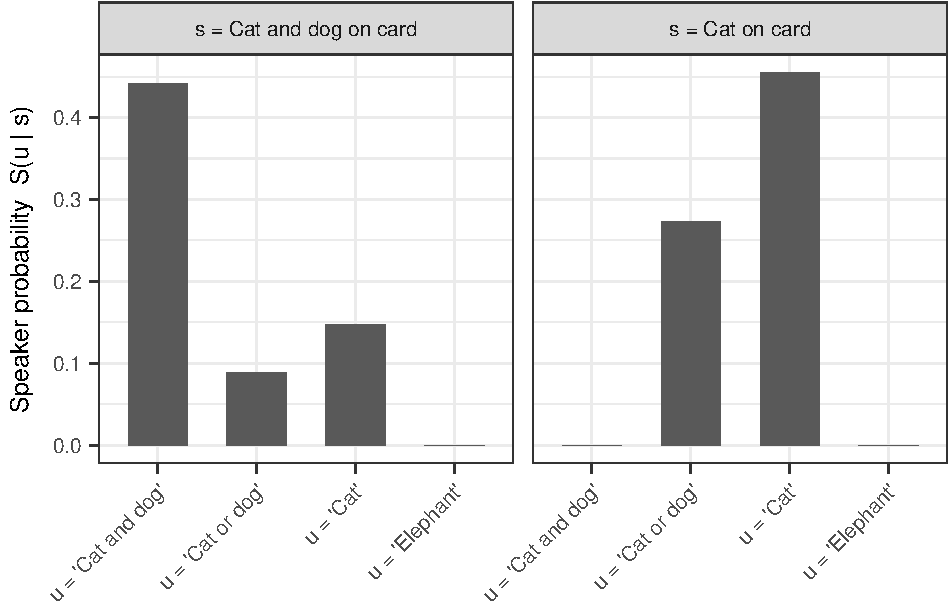
\includegraphics{writeup_files/figure-latex/speakerprobs-1.pdf}
\caption{\label{fig:speakerprobs}Speaker probabilities of utterances on the
exhaustive and scalar trials, as obtained using the model described in
this section.}
\end{figure}

\begin{verbatim}
## <ggproto object: Class ScaleDiscrete, Scale>
##     aesthetics: fill
##     axis_order: function
##     break_info: function
##     break_positions: function
##     breaks: waiver
##     call: call
##     clone: function
##     dimension: function
##     drop: TRUE
##     expand: waiver
##     get_breaks: function
##     get_breaks_minor: function
##     get_labels: function
##     get_limits: function
##     guide: FALSE
##     is_discrete: function
##     is_empty: function
##     labels: waiver
##     limits: NULL
##     make_sec_title: function
##     make_title: function
##     map: function
##     map_df: function
##     n.breaks.cache: NULL
##     na.translate: TRUE
##     na.value: NA
##     name: waiver
##     palette: function
##     palette.cache: NULL
##     position: left
##     range: <ggproto object: Class RangeDiscrete, Range>
##         range: NULL
##         reset: function
##         train: function
##         super:  <ggproto object: Class RangeDiscrete, Range>
##     reset: function
##     scale_name: manual
##     train: function
##     train_df: function
##     transform: function
##     transform_df: function
##     super:  <ggproto object: Class ScaleDiscrete, Scale>
\end{verbatim}

The linking hypothesis under discussion assumes that speaker
probabilities of utterance given meaning are invariant across a) our
four different experimental conditions, b) across participants, and c)
within participants (that is, participants are not capable of updating
their \(S_1\) distribution in a local discourse context). We note that
the assumption (b) may conceivably be relaxed by allowing one or more of
the parameters in the model -- including the prior probability over
world states \(P_w\), the cost function on utterances \(C\), or the
rationality parameter \(\alpha\) -- to vary across participants. We also
note that assumption (c) in particular is in tension with a growing body
of empirical evidence that semantic and pragmatic interpretation is
modulated by rapid adaptation to the linguistic and social features of
one's interlocutors (Fine, Jaeger, Farmer, \& Qian, 2013; Kleinschmidt
\& Jaeger, 2015).

However, if we should like to keep the above assumptions in place, then
we must look elsewhere to explain the observed variation in our
experimental data. In particular, this linking hypothesis, coupled with
our assumptions, commits us to explaining variation in the data in terms
of the threshold parameters of our responder model \(R\). Consider first
the variation in response across different experimental conditions on a
given trial, e.g.~evaluation of a guess of \enquote{cat and dog} when
the card contains both a cat and a dog. The variation in the proportion
of responses of \enquote{right} on this trial between the binary,
ternary, quaternary, and quinary conditions indicates that the threshold
value for \enquote{right} responses must vary across conditions; that
is, we predict that the \(\theta\) of the binary condition will differ
from, e.g., the \(\theta_1\) of the ternary condition as well as the
\(\theta_1\) of the quaternary condition. We also observed variation in
response on this trial within a single condition (for example, a
sizeable minority of participants responded \enquote{wrong} to this
trial in the binary condition). Thus, this linking hypothesis is
committed to the notion that threshold values may vary across
participants, such that a speaker probability of utterance \(S_1\)(u
\textbar{} s) can fall below \(\theta\) for some subset of participants
while \(S_1\)(u \textbar{} s) itself remains constant across
participants.

Lastly, it is conceivable that for two utterances of the same
conditional probability and in the same experimental condition, a
participant in our experiment provided a judgment of, e.g.
\enquote{right} to one utterance but \enquote{wrong} to the other. That
is, it is possible that there was within-subject variation in this
experiment. One way to represent such variation would be to posit that
the parameterization of threshold values proceeds stochastically and
that threshold values are recalibrated for every individual sentence
verification task. Rather than representing a threshold as a discrete
value N between 0 and 1, we can represent that threshold as a
distribution over possible threshold values -- with mass centered around
N. Whenever an individual encounters a sentence verification task, such
as a single trial of our truth value judgment task experiment, the
threshold value is recalibrated by sampling from this distribution. If
we allow values of \(\theta\) to vary as a result of this schotastic
process, for the possibility that \(S_1\)(u \textbar{} s) sometimes
falls below \(\theta\) (and is otherwise above \(\theta\)) for a given
participant.

One outstanding empirical problem is the pattern of response we observed
for \enquote{cat and dog} on trials where there was only a cat on the
card. Because this utterance is strictly false in this world state, it
is surprising -- on both the traditional view as well as on the account
developed here -- that participants assigned this utterance ratings
above \enquote{wrong} with any systematicity. However, this is exactly
what we observed, particulary in the quaternary and quinary conditions
of the experiment, where a sizeable minority of participants considered
this utterance \enquote{kinda right}. As Figure \ref{fig:speakerprobs}
demonstrates, the conditional speaker probability of this utterance in
this world state is 0; thus, there is no conceivable threshold value
that would allow this utterance to ever be rated above \enquote{wrong}
(on the reasonable assumption that the thresholds in our responder model
\(R\) should be nonzero). Any linking hypothesis will have to engage
with this data point, and we leave to future work an analysis which
captures participants' behavior in this condition.

For the time being, however, we present the above analysis as a proof of
concept for the following idea: by relaxing the assumptions of the
traditional view of scalar implicature (namely, that scalar implicatures
either are or are not calculated, and that behavior on sentence
verification tasks directly reflects this binary interpretation
process), we can propose quantitative models of the variation in
behavior we observe in experimental settings. We note that the linking
analysis proposed here is just one in the space of possible analyses
when traditional assumptions about scalar implicature are relaxed. For
example, one might reject this threshold-based analysis in favor of one
whereby responses are the outcomes of sampling on the (pragmatic speaker
or pragmatic listener) probability distributions provided by an RSA
model. We must leave this investigation to future work, but for now we
emphasize that this kind of quantitative, data-driven and systematic
model criticism is made available to researchers in experimental
pragmatics by revising core assumptions about the nature of scalar
implicature. Though we no longer have a crisp notion of scalar
implicature as something that is or is not \enquote{calculated} in
interpretation, we have new flexibility to explicitly discuss
categorical behavior in experimental settings.

Concluding, we have shown in this paper that inferred
\enquote{implicature rate} -- ubiquitous in theoretical and experimental
pragmatics -- as estimated in truth value judgment tasks, depends on
both the number of responses participants are provided with as well as
on the linking hypothesis from proportion of behavioral responses to
\enquote{implicature rate}. We further sketched an alternate linking
hypothesis that treats behavioral responses as the result of
probabilistic reasoning about speakers' likely productions. While a
thorough model comparison is still outstanding, this kind of linking
hypothesis opens a door towards more systematic and rigorous formulation
and testing of linking hypotheses between theoretical notions of
interest in pragmatics and behavioral responses in experimental
paradigms.

\section{References}\label{references}

\setlength{\parindent}{-0.5in} \setlength{\leftskip}{0.5in}

\hypertarget{refs}{}
\hypertarget{ref-Barner2011}{}
Barner, D., Brooks, N., \& Bale, A. (2011). Accessing the unsaid: the
role of scalar alternatives in children's pragmatic inference.
\emph{Cognition}, \emph{118}(1), 84--93.
doi:\href{https://doi.org/10.1016/j.cognition.2010.10.010}{10.1016/j.cognition.2010.10.010}

\hypertarget{ref-barr2013random}{}
Barr, D. J., Levy, R., Scheepers, C., \& Tily, H. J. (2013). Random
effects structure for confirmatory hypothesis testing: Keep it maximal.
\emph{Journal of Memory and Language}, \emph{68}(3), 255--278.

\hypertarget{ref-BenzGotzner2014}{}
Benz, A., \& Gotzner, N. (2014). Embedded implicatures revisited: Issues
with the Truth-Value Judgment Paradigm. In J. Degen, M. Franke, \& N. D.
Goodman (Eds.), \emph{Proceedings of the formal \& experimental
pragmatics workshop, european summer school for language, logic and
information (esslli)} (pp. 1--6). Tübingen.

\hypertarget{ref-Bergen2012}{}
Bergen, L., \& Grodner, D. J. (2012). Speaker knowledge influences the
comprehension of pragmatic inferences. \emph{Journal of Experimental
Psychology. Learning, Memory, and Cognition}, \emph{38}(5), 1450--60.
doi:\href{https://doi.org/10.1037/a0027850}{10.1037/a0027850}

\hypertarget{ref-Bergen2016}{}
Bergen, L., Levy, R., \& Goodman, N. (2016). Pragmatic reasoning through
semantic inference. \emph{Semantics and Pragmatics}, \emph{9}(1984),
1--46. doi:\href{https://doi.org/10.3765/sp.9.20}{10.3765/sp.9.20}

\hypertarget{ref-Bonnefon2009}{}
Bonnefon, J.-F., Feeney, A., \& Villejoubert, G. (2009). When some is
actually all: scalar inferences in face-threatening contexts.
\emph{Cognition}, \emph{112}(2), 249--58.
doi:\href{https://doi.org/10.1016/j.cognition.2009.05.005}{10.1016/j.cognition.2009.05.005}

\hypertarget{ref-Bott2016}{}
Bott, L., \& Chemla, E. (2016). Shared and distinct mechanisms in
deriving linguistic enrichment. \emph{Journal of Memory and Language},
\emph{91}, 117--140.
doi:\href{https://doi.org/10.1016/j.jml.2016.04.004}{10.1016/j.jml.2016.04.004}

\hypertarget{ref-Bott2004}{}
Bott, L., \& Noveck, I. (2004). Some utterances are underinformative:
The onset and time course of scalar inferences. \emph{Journal of Memory
and Language}, \emph{51}(3), 437--457.
doi:\href{https://doi.org/10.1016/j.jml.2004.05.006}{10.1016/j.jml.2004.05.006}

\hypertarget{ref-Breheny2013}{}
Breheny, R., Ferguson, H. J., \& Katsos, N. (2013). Taking the epistemic
step: Toward a model of on-line access to conversational implicatures.
\emph{Cognition}, \emph{126}(3), 423--40.
doi:\href{https://doi.org/10.1016/j.cognition.2012.11.012}{10.1016/j.cognition.2012.11.012}

\hypertarget{ref-Breheny2006}{}
Breheny, R., Katsos, N., \& Williams, J. (2006). Are generalised scalar
implicatures generated by default? An on-line investigation into the
role of context in generating pragmatic inferences. \emph{Cognition},
\emph{100}(3), 434--63.
doi:\href{https://doi.org/10.1016/j.cognition.2005.07.003}{10.1016/j.cognition.2005.07.003}

\hypertarget{ref-burkner2016brms}{}
Bürkner, P.-C., \& others. (2016). Brms: An r package for bayesian
multilevel models using stan. \emph{Journal of Statistical Software},
\emph{80}(1), 1--28.

\hypertarget{ref-Chemla2011}{}
Chemla, E., \& Spector, B. (2011). Experimental Evidence for Embedded
Scalar Implicatures. \emph{Journal of Semantics}, \emph{28}(3),
359--400.

\hypertarget{ref-chierchia2001}{}
Chierchia, G., Crain, S., Teresa, M., Guasti, M. T., Gualmini, A., \&
Meroni, L. (2001). The Acquisition of Disjunction: Evidence for a
Grammatical View of Scalar Implicatures. In A. H.-J. D. Et al. (Ed.),
\emph{BUCLD 25 proceedings} (pp. 157--168). Somerville, MA: Cascadilla
Press.

\hypertarget{ref-DeNeys2007}{}
De Neys, W., \& Schaeken, W. (2007). When People Are More Logical Under
Cognitive Load - Dual Task Impact on Scalar Implicature.
\emph{Experimental Psychology}, \emph{54}(2), 128--133.
doi:\href{https://doi.org/10.1027/1618-3169.54.2.128}{10.1027/1618-3169.54.2.128}

\hypertarget{ref-Degen2015}{}
Degen, J. (2015). Investigating the distribution of 'some' (but not
'all') implicatures using corpora and web-based methods. \emph{Semantics
and Pragmatics}, \emph{8}(11), 1--55.
doi:\href{https://doi.org/10.3765/sp.8.11}{10.3765/sp.8.11}

\hypertarget{ref-Degen2014}{}
Degen, J., \& Goodman, N. D. (2014). Lost your marbles? The puzzle of
dependent measures in experimental pragmatics. \emph{Proceedings of the
36th Annual Conference of the Cognitive Science Society}, 397--402.

\hypertarget{ref-DegenTanenhaus2015}{}
Degen, J., \& Tanenhaus, M. K. (2015). Processing scalar implicature A
constraint-based approach. \emph{Cognitive Science}, \emph{39}(4),
667--710.
doi:\href{https://doi.org/10.1111/cogs.12171}{10.1111/cogs.12171}

\hypertarget{ref-DegenTanenhaus2016}{}
Degen, J., \& Tanenhaus, M. K. (2016). Availability of Alternatives and
the Processing of Scalar Implicatures: A Visual World Eye-Tracking
Study. \emph{Cognitive Science}, \emph{40}(1), 172--201.
doi:\href{https://doi.org/10.1111/cogs.12227}{10.1111/cogs.12227}

\hypertarget{ref-Degen2013}{}
Degen, J., Franke, M., \& Jäger, G. (2013). Cost-Based Pragmatic
Inference about Referential Expressions. \emph{Proceedings of the 35th
Annual Conference of the Cognitive Science Society (CogSci'13)},
376--281.

\hypertarget{ref-DegenTG2015}{}
Degen, J., Tessler, M. H., \& Goodman, N. D. (2015). Wonky worlds:
Listeners revise world knowledge when utterances are odd.
\emph{Proceedings of the 37th Annual Conference of the Cognitive Science
Society}, (2), 548--553.

\hypertarget{ref-Doran2012}{}
Doran, R., Ward, G., Larson, M., McNabb, Y., \& Baker, R. E. (2012). A
novel experimental paradigm for distinguishing between what is said and
what is implicated. \emph{Language}, \emph{88}, 124--154.

\hypertarget{ref-Fine2013}{}
Fine, A. B., Jaeger, T. F., Farmer, T. F., \& Qian, T. (2013). Rapid
expectation adaptation during syntactic comprehension. \emph{PLoS ONE},
\emph{8}(10).
doi:\href{https://doi.org/10.1371/\%20journal.pone.0077661}{10.1371/ journal.pone.0077661}

\hypertarget{ref-Frank2012}{}
Frank, M. C., \& Goodman, N. D. (2012). Predicting pragmatic reasoning
in language games. \emph{Science}, \emph{336}, 998.

\hypertarget{ref-Franke2016}{}
Franke, M., \& Jäger, G. (2016). Probabilistic pragmatics, or why Bayes
' rule is probably important for pragmatics. \emph{Zeitschrift Für
Sprachwissenschaft}, \emph{35}(1), 3--44.

\hypertarget{ref-Geurts2010}{}
Geurts, B. (2010). \emph{Quantity implicatures}. Cambridge: Cambridge
Univ Press.

\hypertarget{ref-Geurts2009}{}
Geurts, B., \& Pouscoulous, N. (2009). Embedded implicatures?!?
\emph{Semantics and Pragmatics}, \emph{2}, 1--34.
doi:\href{https://doi.org/10.3765/sp.2.4}{10.3765/sp.2.4}

\hypertarget{ref-Goodman2016}{}
Goodman, N. D., \& Frank, M. C. (2016). Pragmatic Language
Interpretation as Probabilistic Inference. \emph{Trends in Cognitive
Sciences}, \emph{20}(11), 818--829.
doi:\href{https://doi.org/10.1016/j.tics.2016.08.005}{10.1016/j.tics.2016.08.005}

\hypertarget{ref-Goodman2013}{}
Goodman, N. D., \& Stuhlmüller, A. (2013). Knowledge and implicature:
modeling language understanding as social cognition. \emph{Topics in
Cognitive Science}, \emph{5}(1), 173--84.
doi:\href{https://doi.org/10.1111/tops.12007}{10.1111/tops.12007}

\hypertarget{ref-grice1975}{}
Grice, H. P. (1975). Logic and Conversation. \emph{Syntax and
Semantics}, \emph{3}, 41--58. Retrieved from
\href{http://books.google.com/books?hl=en\%7B/\&\%7Dlr=\%7B/\&\%7Did=hQCzOmaGeVYC\%7B/\&\%7Doi=fnd\%7B/\&\%7Dpg=PA121\%7B/\&\%7Ddq=Logic+and+conversation\%7B/\&\%7Dots=j7aijUymwm\%7B/\&\%7Dsig=iV1rz1eEm4ns6bQ6CevIURXFVO4}{http://books.google.com/books?hl=en\{\textbackslash{}\&\}lr=\{\textbackslash{}\&\}id=hQCzOmaGeVYC\{\textbackslash{}\&\}oi=fnd\{\textbackslash{}\&\}pg=PA121\{\textbackslash{}\&\}dq=Logic+and+conversation\{\textbackslash{}\&\}ots=j7aijUymwm\{\textbackslash{}\&\}sig=iV1rz1eEm4ns6bQ6CevIURXFVO4}

\hypertarget{ref-Grodner2010}{}
Grodner, D. J., Klein, N. M., Carbary, K. M., \& Tanenhaus, M. K.
(2010). ``Some,'' and possibly all, scalar inferences are not delayed:
Evidence for immediate pragmatic enrichment. \emph{Cognition},
\emph{116}(1), 42--55.
doi:\href{https://doi.org/10.1016/j.cognition.2010.03.014}{10.1016/j.cognition.2010.03.014}

\hypertarget{ref-Hirschberg1985}{}
Hirschberg, J. (1985). \emph{A Theory of Scalar Implicature} (PhD thesis
No. MS-CIS-85-56). University of Pennsylvania; Garland Publishing
Company.

\hypertarget{ref-Horn1972}{}
Horn, L. (1972). \emph{On the Semantic Properties of the Logical
Operators in English} (PhD thesis). UCLA.

\hypertarget{ref-horn1984}{}
Horn, L. (1984). Toward a new taxonomy for pragmatic inference: Q-based
and R-based implicature. In D. Schiffrin (Ed.), \emph{Meaning, form, and
use in context: Linguistic applications} (pp. 11--42). Washington:
Georgetown University Press.

\hypertarget{ref-Horowitz2017}{}
Horowitz, A. C., Schneider, R. M., \& Frank, M. C. (2017). The Trouble
With Quantifiers: Exploring Children's Deficits in Scalar Implicature.
\emph{Child Development}, 1--40.
doi:\href{https://doi.org/10.1111/cdev.13014}{10.1111/cdev.13014}

\hypertarget{ref-huang2009}{}
Huang, Y. T., \& Snedeker, J. (2009). On-line interpretationf of scalar
quantifiers: Insight into the semantics-pragmatics interface.
\emph{Cognitive Psychology}, \emph{58}, 376--415.

\hypertarget{ref-Kao2014}{}
Kao, J., Wu, J., Bergen, L., \& Goodman, N. D. (2014). Nonliteral
understanding of number words. \emph{Proceedings of the National Academy
of Sciences of the United States of America}, \emph{111}(33),
12002--12007.
doi:\href{https://doi.org/10.1073/pnas.1407479111}{10.1073/pnas.1407479111}

\hypertarget{ref-Katsos2011}{}
Katsos, N., \& Bishop, D. V. M. (2011). Pragmatic tolerance:
implications for the acquisition of informativeness and implicature.
\emph{Cognition}, \emph{120}(1), 67--81.
doi:\href{https://doi.org/10.1016/j.cognition.2011.02.015}{10.1016/j.cognition.2011.02.015}

\hypertarget{ref-Kleinschmidt2015}{}
Kleinschmidt, D. F., \& Jaeger, T. F. (2015). Robust speech perception:
Recognize the familiar, generalize to the similar, and adapt to the
novel. \emph{Psychological Review}, \emph{122}(2), 148--203.
doi:\href{https://doi.org/10.1037/a0038695}{10.1037/a0038695}

\hypertarget{ref-levinson2000}{}
Levinson, S. C. (2000). \emph{Presumptive Meanings - The Theory of
Generalized Conversational Implicature}. MIT Press.

\hypertarget{ref-DeMarneffe2017}{}
Marneffe, M.-C. de, \& Tonhauser, J. (2016). Inferring meaning from
indirect answers to polar questions: The contribution of the
rise-fall-rise contour. In E. Onea, M. Zimmermann, \& K. von Heusinger
(Eds.), \emph{Questions in discourse}. Leiden: Brill Publishing.

\hypertarget{ref-Musolino2004}{}
Musolino, J. (2004). The semantics and acquisition of number words:
integrating linguistic and developmental perspectives. \emph{Cognition},
\emph{93}(1), 1--41.
doi:\href{https://doi.org/10.1016/j.cognition.2003.10.002}{10.1016/j.cognition.2003.10.002}

\hypertarget{ref-Noveck2001}{}
Noveck, I. (2001). When children are more logical than adults:
experimental investigations of scalar implicature. \emph{Cognition},
\emph{78}(2), 165--188. Retrieved from
\url{http://www.ncbi.nlm.nih.gov/pubmed/11074249}

\hypertarget{ref-noveck2008}{}
Noveck, I. A., \& Reboul, A. (2008). Experimental pragmatics: a Gricean
turn in the study of language. \emph{Trends in Cognitive Sciences},
\emph{12}(11), 425--431.
doi:\href{https://doi.org/10.1016/j.tics.2008.07.009}{10.1016/j.tics.2008.07.009}

\hypertarget{ref-Noveck2003}{}
Noveck, I., \& Posada, A. (2003). Characterizing the Time Course of an
Implicature: an Evoked Potentials Study. \emph{Brain and Language},
\emph{85}(2), 203--210.
doi:\href{https://doi.org/10.1016/S0093-934X(03)00053-1}{10.1016/S0093-934X(03)00053-1}

\hypertarget{ref-Papafragou2004}{}
Papafragou, A., \& Tantalou, N. (2004). Children's Computation of
Implicatures. \emph{Language Acquisition}, \emph{12}(1), 71--82.

\hypertarget{ref-Politzer-Ahles2013}{}
Politzer-Ahles, S., \& Fiorentino, R. (2013). The Realization of Scalar
Inferences: Context Sensitivity without Processing Cost. \emph{PLoS
ONE}, \emph{8}(5).
doi:\href{https://doi.org/10.1371/journal.pone.0063943}{10.1371/journal.pone.0063943}

\hypertarget{ref-Potts2015}{}
Potts, C., Lassiter, D., Levy, R., \& Frank, M. C. (2015). Embedded
implicatures as pragmatic inferences under compositional lexical
uncertainty. \emph{Journal of Semantics}, \emph{33}(1975), 755--802.
doi:\href{https://doi.org/10.1093/jos/ffv012}{10.1093/jos/ffv012}

\hypertarget{ref-Qing2015}{}
Qing, C., \& Franke, M. (2015). Variations on a bayesian theme:
Comparing bayesian models of referential reasoning. In H. Zeevat \&
H.-C. Schmitz (Eds.), \emph{Bayesian natural language semantics and
pragmatics} (Vol. 2, pp. 201--220). Cham, Switzerland: Springer
International Publishing.
doi:\href{https://doi.org/10.1007/978-3-319-17064-0_9}{10.1007/978-3-319-17064-0\_9}

\hypertarget{ref-Scontras2017}{}
Scontras, G., Degen, J., \& Goodman, N. D. (2017). Subjectivity predicts
adjective ordering preferences. \emph{Open Mind: Discoveries in
Cognitive Science}, \emph{1}(1), 53--65.
doi:\href{https://doi.org/10.1162/opmi}{10.1162/opmi}

\hypertarget{ref-Stiller2015}{}
Stiller, A. J., Goodman, N. D., \& Frank, M. C. (2015). Ad-hoc
Implicature in Preschool Children. \emph{Language Learning and
Development}, \emph{11}(2), 176--190.
doi:\href{https://doi.org/10.1080/15475441.2014.927328}{10.1080/15475441.2014.927328}

\hypertarget{ref-Tanenhaus2004}{}
Tanenhaus, M. K. (2004). On-line sentence processing: past, present and
future. In M. Carreiras \& C. Clifton (Eds.), \emph{On-line sentence
processing: ERPS, eye movements and beyond} (pp. 371--392). London, UK:
Psychology Press.

\hypertarget{ref-VanTiel2014}{}
Tiel, B. van, Miltenburg, E. van, Zevakhina, N., \& Geurts, B. (2014).
Scalar diversity. \emph{Journal of Semantics}.
doi:\href{https://doi.org/10.1093/jos/ffu017}{10.1093/jos/ffu017}

\hypertarget{ref-Tomlinson2013}{}
Tomlinson, J. M., Bailey, T. M., \& Bott, L. (2013). Possibly all of
that and then some: Scalar implicatures are understood in two steps.
\emph{Journal of Memory and Language}, \emph{69}(1), 18--35.
doi:\href{https://doi.org/10.1016/j.jml.2013.02.003}{10.1016/j.jml.2013.02.003}

\hypertarget{ref-Zondervan2010}{}
Zondervan, A. (2010). \emph{Scalar implicatures or focus: an
experimental approach} (PhD thesis). Universiteit Utrecht, Amsterdam.






\end{document}
